\documentclass[twocolumn, traditabstract]{aa}  

\usepackage{fixltx2e}
\usepackage[english]{babel}
\usepackage{graphicx,amsmath}
\usepackage{epstopdf}
\usepackage{epsf,color}
\usepackage[mathscr]{eucal}
\usepackage{amsmath}
\usepackage{amssymb,amsfonts}
\usepackage{natbib}
\usepackage{txfonts}
\usepackage{dsfont}
\definecolor{Mygreen}{rgb}{0.00, 0.72, 0.0}
\definecolor{Mypink}{rgb}{1.0, 0.0, 0.5}
\usepackage[breaklinks, citecolor=blue, linkcolor=Mygreen, urlcolor=Mypink, colorlinks=true, debug, baseurl=' ']{hyperref}
\usepackage{float}
\usepackage{color}
\usepackage{scrextend}
\usepackage{nccmath}
\usepackage{mathtools, cuted}
\usepackage{lscape}
%\usepackage{widetext}
\usepackage{flushend}
\usepackage[T1]{fontenc}
\usepackage{gensymb}
\usepackage{diagbox}



\newcommand{\nika}{{\it NIKA}}
\newcommand{\nikad}{{\it NIKA2}}
\newcommand{\Q}{$Q$}
\newcommand{\I}{$I$}
\newcommand{\U}{$U$}
\newcommand{\di}{$dI$}
\newcommand{\dq}{$dQ$}
\newcommand{\eps}{$\varepsilon$}
\newcommand{\epsCMB}{$\varepsilon_{CMB}$}
\newcommand{\epsDET}{$\varepsilon_{det}$}
\newcommand{\rf}{{\it RfdIdQ}}
\newcommand{\cf}{{\it Cf}}


\def\simlt{\lower.5ex\hbox{$\; \buildrel < \over \sim \;$}}
\def\simgt{\lower.5ex\hbox{$\; \buildrel > \over \sim \;$}}
\def\NIKA{\textit{NIKA}}

\bibpunct{(}{)}{;}{a}{}{,}
\bibliographystyle{aa}

\begin{document}
\title{KID systematics and CMB polarization blabla}
%\author{R.~Adam \inst{\ref{OCA},\ref{LPSC},\ref{CEFCA}}\thanks{Corresponding author: R\'emi Adam, \url{remi.adam@oca.eu}}
\and O.~Hahn\inst{\ref{OCA}}						%NCT
\and  F.~Ruppin \inst{\ref{LPSC}}
\and  P.~Ade \inst{\ref{Cardiff}}
\and  P.~Andr\'e \inst{\ref{CEA}}
\and M.~Arnaud\inst{\ref{CEA}}					%NCT
\and I.~Bartalucci\inst{\ref{CEA}}					%NCT
\and  A.~Beelen \inst{\ref{IAS}}
\and  A.~Beno\^it \inst{\ref{Neel}}
\and  A.~Bideaud \inst{\ref{Neel}}
\and  N.~Billot \inst{\ref{IRAME}}
\and  O.~Bourrion \inst{\ref{LPSC}}
\and  M.~Calvo \inst{\ref{Neel}}
\and  A.~Catalano \inst{\ref{LPSC}}
\and  G.~Coiffard \inst{\ref{IRAMF}}
\and  B.~Comis \inst{\ref{LPSC}}
\and  A.~D'Addabbo \inst{\ref{Neel},\ref{Roma}}
\and  F.-X.~D\'esert \inst{\ref{IPAG}}
\and  S.~Doyle \inst{\ref{Cardiff}}
\and C.~Ferrari\inst{\ref{OCA}}						%NCT
\and  J.~Goupy \inst{\ref{Neel}}
\and  C.~Kramer \inst{\ref{IRAME}}
\and  G.~Lagache \inst{\ref{LAM}}
\and  S.~Leclercq \inst{\ref{IRAMF}}
\and  J.-F.~Lestrade \inst{\ref{LERMA}}
\and  J.F.~Mac\'ias-P\'erez \inst{\ref{LPSC}}
\and G.~Martinez Aviles\inst{\ref{OCA}}				%NCT
\and D.~Martizzi\inst{\ref{Berkeley}}					%NCT
\and S.~Maurogordato\inst{\ref{OCA}}				%NCT
\and  P.~Mauskopf \inst{\ref{Cardiff},\ref{Arizona}}
\and  F.~Mayet \inst{\ref{LPSC}}
\and  A.~Monfardini \inst{\ref{Neel}}
\and  F.~Pajot \inst{\ref{IAS}}
\and  E.~Pascale \inst{\ref{Cardiff}}
\and  L.~Perotto \inst{\ref{LPSC}}
\and  G.~Pisano \inst{\ref{Cardiff}}
\and E.~Pointecouteau\inst{\ref{IRAP}, \ref{UniToulouse}}%NCT
\and  N.~Ponthieu \inst{\ref{IPAG}}
\and G.W.~Pratt\inst{\ref{CEA}}					%NCT
\and  V.~Rev\'eret \inst{\ref{CEA}}
\and M.~Ricci\inst{\ref{OCA}}						%NCT
\and  A.~Ritacco \inst{\ref{IRAME}}
\and  L.~Rodriguez \inst{\ref{CEA}}
\and  C.~Romero \inst{\ref{IRAMF}}
\and  H.~Roussel \inst{\ref{IAP}}
\and  K.~Schuster \inst{\ref{IRAMF}}
\and  A.~Sievers \inst{\ref{IRAME}}
\and  S.~Triqueneaux \inst{\ref{Neel}}
\and  C.~Tucker \inst{\ref{Cardiff}}
\and H.-Y.~Wu\inst{\ref{CalTech}}					%NCT
\and  R.~Zylka \inst{\ref{IRAMF}}}

\institute{
  Laboratoire Lagrange, Universit\'e C\^ote d'Azur, Observatoire de la C\^ote d'Azur, CNRS, Blvd de l'Observatoire, CS 34229, 06304 Nice cedex 4, France
  \label{OCA}
  \and
  Laboratoire de Physique Subatomique et de Cosmologie, Universit\'e Grenoble Alpes, CNRS/IN2P3, 53, avenue des Martyrs, Grenoble, France
  \label{LPSC}
    \and
  Centro de Estudios de F\'isica del Cosmos de Arag\'on (CEFCA), Plaza San Juan, 1, planta 2, E-44001, Teruel, Spain
  \label{CEFCA}
  \and
Institut de RadioAstronomie Millim\'etrique (IRAM), Grenoble, France
  \label{IRAMF}
\and
Laboratoire AIM, CEA/IRFU, CNRS/INSU, Universit\'e Paris Diderot, CEA-Saclay, 91191 Gif-Sur-Yvette, France 
  \label{CEA}
\and
Astronomy Instrumentation Group, University of Cardiff, UK
  \label{Cardiff}
\and
Institut d'Astrophysique Spatiale (IAS), CNRS and Universit\'e Paris Sud, Orsay, France
  \label{IAS}
\and
Institut N\'eel, CNRS and Universit\'e Grenoble Alpes, France
  \label{Neel}
\and
Institut de RadioAstronomie Millim\'etrique (IRAM), Granada, Spain
  \label{IRAME}
\and
Dipartimento di Fisica, Sapienza Universit\`a di Roma, Piazzale Aldo Moro 5, I-00185 Roma, Italy
  \label{Roma}
\and
Univ. Grenoble Alpes, CNRS, IPAG, F-38000 Grenoble, France 
  \label{IPAG}
    \and
Aix Marseille Universit\'e, CNRS, LAM (Laboratoire d'Astrophysique de Marseille) UMR 7326, 13388, Marseille, France
  \label{LAM}
\and
School of Earth and Space Exploration and Department of Physics, Arizona State University, Tempe, AZ 85287
  \label{Arizona}
\and
Universit\'e de Toulouse, UPS-OMP, Institut de Recherche en Astrophysique et Plan\'etologie (IRAP), Toulouse, France
  \label{IRAP}
\and
CNRS, IRAP, 9 Av. colonel Roche, BP 44346, F-31028 Toulouse cedex 4, France 
  \label{IRAP2}
\and
University College London, Department of Physics and Astronomy, Gower Street, London WC1E 6BT, UK
  \label{UCL}
\and 
Institut d'Astrophysique de Paris, Sorbonne Universit\'es, UPMC Univ. Paris 06, CNRS UMR 7095, 75014 Paris, France 
  \label{IAP}
\and 
LERMA, CNRS, Observatoire de Paris, 61 avenue de l'Observatoire, Paris, France
  \label{LERMA}
  \and  
Department of Astronomy, University of California, Berkeley, CA 94720-3411, USA
  \label{Berkeley}
    \and
Universit\'e de Toulouse, UPS-OMP, Institut de Recherche en Astrophysique et Plan\'etologie (IRAP), Toulouse, France
  \label{IRAP}
\and
CNRS, IRAP, 9 Av. colonel Roche, BP 44346, F-31028 Toulouse cedex 4, France 
  \label{UniToulouse}
  \and
California Institute of Technology, MC 367-17, Pasadena, CA 91125, USA.
  \label{CalTech}  
}


\date{Received \today \ / Accepted --}
	
\abstract{Here goes the abstract}
\titlerunning{KIDs systematics}
\authorrunning{TBD}
\keywords{Techniques: polarization -- KIDs --  individual: NIKA }
\tableofcontents
\maketitle

\section{Introduction}
\label{sec:introduction}

%Pour citer les papiers: \citep{planck2013mission} ou alors
%\citep{2010A&A...518L.100M,arzoumianian}.


%\begin{itemize}
%\item Why we want to measure CMB polarization B modes
%\item The need for matrices and the KID solution, quickly mention other
%  solutions and multiplexing
%\item Importance to master systematic effects (ref. to previous papers)
%\item KIDs are a new technology that has not yet reached a ``space proof''
%  maturity. In this paper, we address a few specific systematics to KIDs.
%\item Outline
%\end{itemize}

The measurement of CMB polarization, and especially the detection of $B$ modes, is
one of the major challenges in modern cosmology. In fact, a key motivation for
CMB polarization measurements is the theory of cosmic inflation. $B$ modes can be
generated by two mechanisms : gravitational lensing of $E$ modes
\citep{2013PhRvL.111n1301H}, or by gravitational waves produced during
inflation. The detection of primordial B modes would represent an indirect
detection of primordial gravitational waves, and as a result, establish the
theory of cosmic inflation.\\ In order to detect B modes, we need to study the
universe at high sensitivity. To do so, the development of
large detectors arrays is required.  The most used kind of detectors are
bolometers named Transition Edge Sensors (TES), but now their performances are
limited by the photon noise. It is possible to do medium-sized arrays of TES
detectors (1000 pixels), but developing larger arrays gets complicated for
technical and economical reasons. Other detectors used are Cold Electron
Bolometer (CEB) \citep{2007stt..conf...93K} and Superconducting Tunnel Junctions
(STJ) but they face difficulties in the fabrication process making them not
suitable for large arrays. Bolometers have enjoyed considerable technical
improvements but further array scaling is strongly limited by the multiplexing
factor of the readout electronics, consequently it was necessary to develop
detectors adapted to strong frequency domain multiplexing.\\ In this context, a
new kind of detectors was developed : the Kinetic Inductance Detectors (KIDs),
proposed by \citet{2003Natur.425..817D}. Since 2007, these detectors have been
developed for the construction of NIKA2 and its prototype NIKA (New IRAM Kids
Arrays), which is the first operational instrument using KIDs
\citep{2010A&A...521A..29M,2016JLTP..184..816C}. The main characteristic that
makes KIDs one of the best candidates to large size detector array is their
natural multiplexing capability. Indeed, the resonant frequencies of a resonator
can be easily controlled during the array design, and the sharpness of the
resonances allows many resonators to be placed into a limited band-width. Thus,
a large number of resonators, can be coupled to a single transmission line, each
one resonating at a different frequency $f_{0}^{i}$ \citep{2010A&A...521A..29M,
  Calvo2008}.\\ Together with high sensitivity, a strict control of systematic effects must be achieved. In fact, due to its faintness, The B-mode polarization can be easily degraded by various systematic
effects and it is important to remove these spurious contributions. Some of
these effects can be reduced in the design of the instruments while others have
to be simulated and corrected a posteriori. Numerous systematic effects arise
from optical and instrumental imperfections, temperature drifts of the optics
and detectors, contaminations by astrophysical foregrounds and te detector
non-linearity. These effects can be modelled and characterized by the spurious
signal $C_{l}$ they produce. For more details see \citep{2008PhRvD..77h3003S,
  quickpol} and references therein.\\ KIDs are a new technology that are now
routinely used in ground-based telescopes. However, in view of futur
uses above the atmosphere, we still have to demonstrate their
compatibility with a space mission (such as COrE \citep{2016arXiv160907263D}),
hence the need to master their sytematic effects. In this paper, we adress a few
specific systematics to KIDs. The paper is organized as follows:
Sect. \ref{sec2} presents a brief description of KIDs...

\section{Overview of KIDs}
\label{sec2}
\subsection{KID physics}

Kinetic inductance detectors are a novel superconducting detector technology that provides high sensitivity and ease of multiplexing. In this section we give a brief summary of the main features of KIDs.\\
KIDs are RLC superconducting resonators made from a thin metal film that react to an incoming radiation by changing their electromagnetic properties. In fact, when photons are absorbed by the superconducting film, they break Cooper pairs and change the ratio of paired (Cooper pair) and unpaired (quasi-particles) charge carriers. The breaking of Cooper pairs increases the quasi-particles density, which causes a change in the kinetic inductance $L_{k}$. This produces a shift of the resonant frequency of the KID \citep{2013A&A...551L..12C}. The absorbed optical power $P_{opt}$ can be directly related to the change in the resonant frequency $\delta f_{0}$, as the relationship between them is linear for small variations in $P_{opt}$ \citep{2010ApPhL..96z3511S}. The operating principle is represented in fig \ref{resonance}.\\

\begin{figure}[h]
\center
	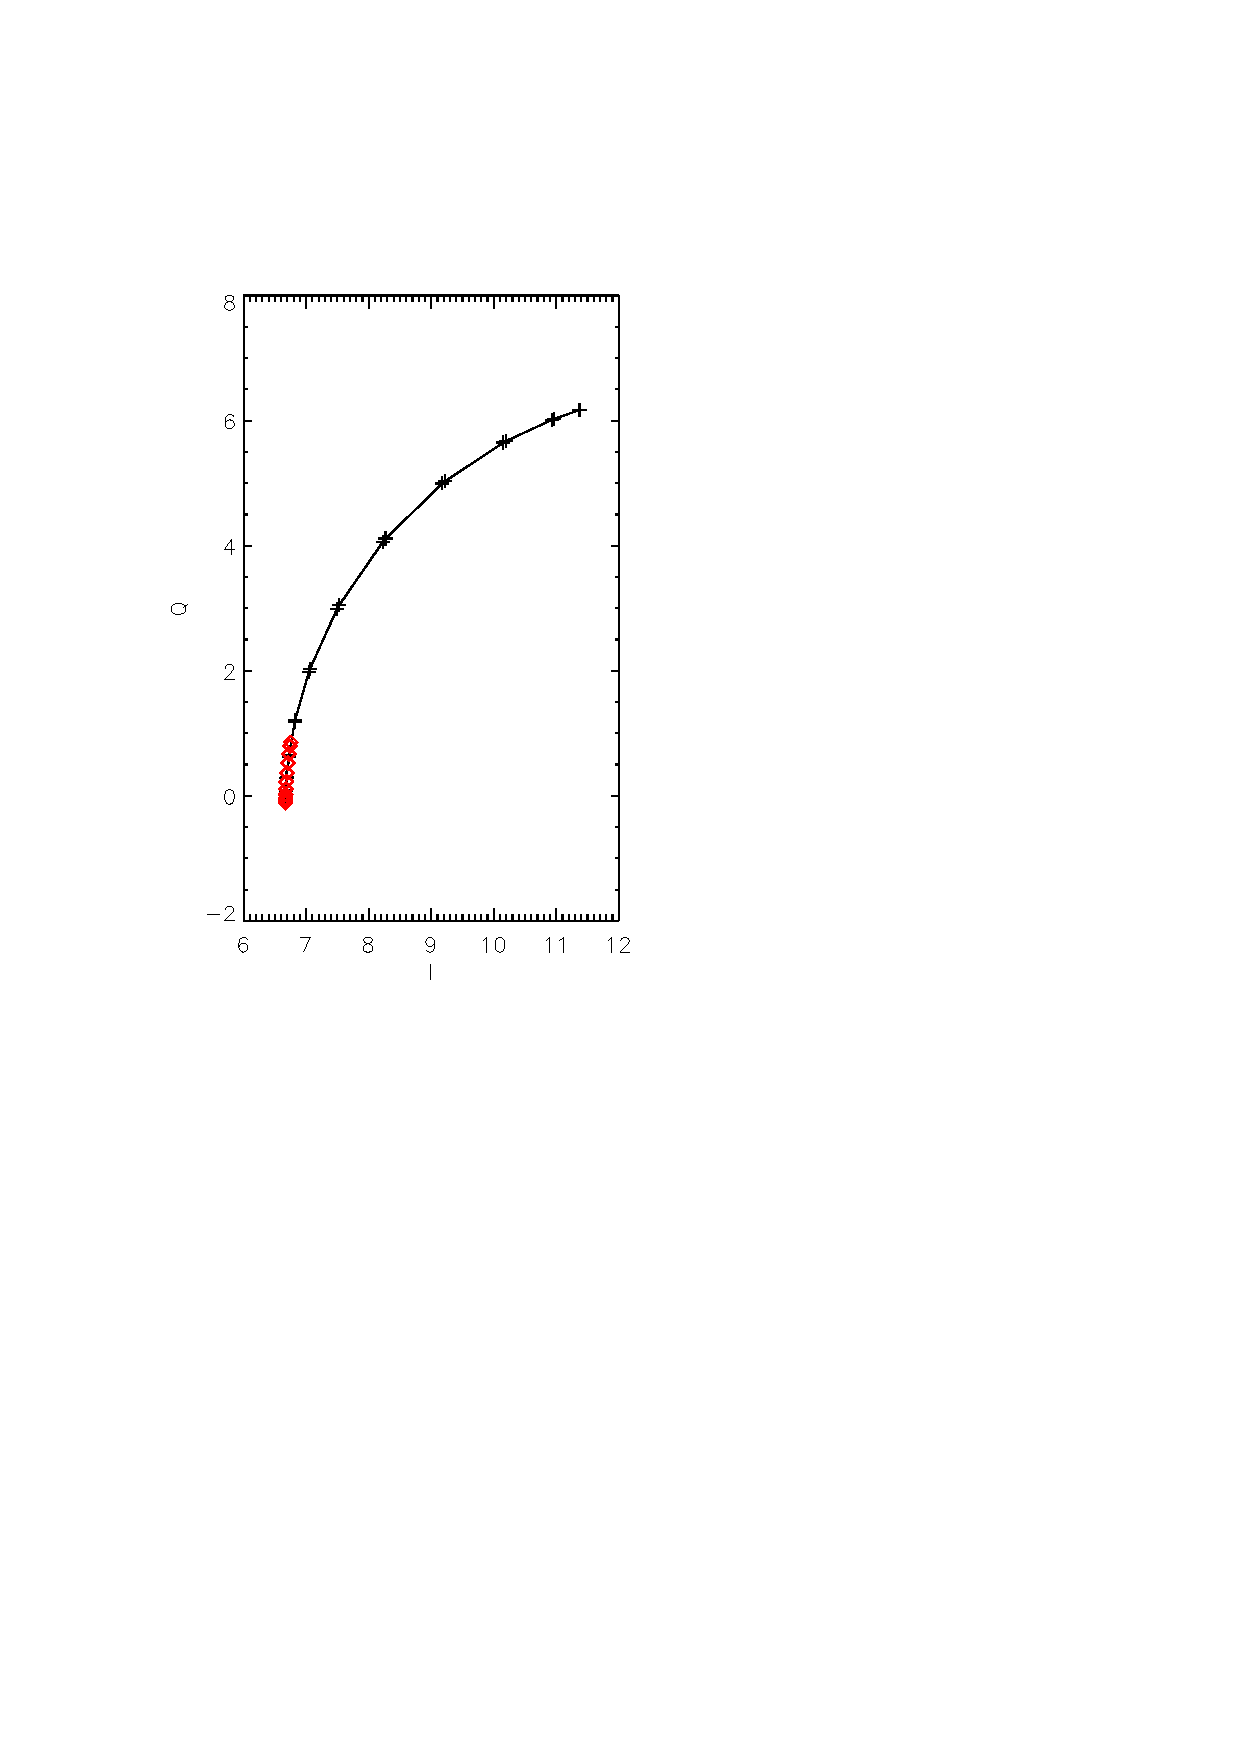
\includegraphics[scale=0.4]{Figures/resonance.png}
	\caption{Schematic representation of a KID resonance in amplitude (left) and phase (right), as a function of the excited tone injected in the feedline. The optical power absorbed by the detector is weak for black curves and increases for red curves. The absorption of a photon shifts the resonance frequency and this is directly proportional to the received power.}
	\label{resonance}
\end{figure}

The KID transfer function is given by :

\begin{equation}
S_{21}(f) = I +jQ .
\end{equation}

where \I  and \Q  give respectively the real (in phase) and imaginary (quadrature) part of the ratio between the input and output signal of the feedline transmission. \\

\subsection{KID model}

In order to model the way a KID reacts to an incoming radiation, we calculate the KID transfer function by following the
parametrisation proposed by \citet{2008ApPhL..93m4102G} :

\begin{equation}
S_{21} = \frac{2Z_{res}Z_{0}}{Z_{res}[2Z_{0} + j(X_{1}+X_{2})] + (Z_{0} +jX_{1})(Z_{0} +jX_{2})},
\end{equation}

with :

\begin{equation}
Z_{res} = \frac{Z_{0}Q_{e}}{2Q_{i}}[1 + 2jQ_{i}\frac{(f-f_{0})}{f_{0}}].
\end{equation}

Where $X_{1}$, $X_{2}$, $Z_{0}$ are impedances, $Q_{i}$ is the intrinsic quality factor of the resonator and $Q_{e}$ is the external quality factor due to coupling with the measurement electronics. $f$ is the frequency of excitation to which the detector is submitted, and $f_{0}$ represents the resonant frequency.  We choose typical values of KIDs $X_{1} = X_{2} = 3 $ $\Omega $, $Z_{0} = 50$ $\Omega$, $Q_{i} \simeq 5.10^{4}$, $Q_{e} \simeq 2.10^{4}$ and $f_{0} = 1.273$x$10^{9}$ Hz.\\

In this paper we use this model to simulate the response of a KID when submitted to different sources of radiation. In order to reconstruct the signal given by a KID, two methods were developed and are presented in the following section.

\section{Methods of signal reconstruction}
\label{sec:signal}


{\bf Unlike the resistance of bolometers that can be directly measured to return
  a signal proportionnal to the incicent power, the monitoring of the evolution
  of the resistance of a KID requires a more complex readout scheme.}

One of the most difficult challenges of operationg a KID is to convert the
\I(t) and \Q(t) values to an absorbed optical power or shift in resonant
frequency as a function of time $\delta f_{0} \propto \delta P_{opt}$. In this
section, we will see how to adress this problem by using a new modulated readout
technique and then by using two different signal reconstruction methods : RfdIdQ
and Cf.

\subsection{Modulated readout technique}
An innovative readout technique has been developed to monitor the change of the signal $\frac{dI}{df}$,$\frac{dQ}{df}$ by using a known frequency shift. This scheme allows continuous simultaneous tracking of KID resonant frequency which change proportionally to the absorbed optical power. To do so, the standart excitation of the detectors which uses a fixed tone is replaced by a new excitation based on two different frequencies. In fact, in order to generate two tones, we modulate the local oscillator signal between two values, separated by $\delta f_{LO} \simeq 1$ kHz, and obtain $f_{+} = f_{0} + \frac{\delta f_{LO}}{2}$ and $f_{-} = f_{0} - \frac{\delta f_{LO}}{2}$ with $f_{0}$ the detector resonant frequency.\\
The values ($I(t)$,$Q(t)$) are then given by :

\begin{equation}
(I(t),Q(t)) = (\frac{I(f_{+}) + I(f_{-})}{2}, \frac{Q(f_{+}) + Q(f_{-})}{2})
\end{equation}

and the differential values are :

\begin{equation}
\label{gradient}
(\frac{dI}{df}(t),\frac{dQ}{df}(t)) = (\frac{I(f_{+}) - I(f_{-})}{\delta f_{LO}}, \frac{Q(f_{+}) - Q(f_{-})}{\delta f_{LO}})
\end{equation}

\begin{figure}[h]
\center
	\includegraphics[scale=0.5]{Figures/resonance-circle.png}
	\caption{Representation in the I-Q plane of a sweep around a resonance. The red line represents the $(I,Q)$ data of the frequency sweep around the resonance.The arrows reprsents ($\frac{dI}{df}$,$\frac{dQ}{df}$). \citep{2013A&A...551L..12C}}
	\label{circle-iq}
\end{figure}

Fig. \ref{circle-iq} shows a typical KID resonance circle. Thanks to this
modulation technique, we obtain four quantities : I, Q and their variation
$\delta I$, $\delta Q$.\\ In this paper, I(t) and Q(t) are sampled at 22 Hz,
they are the mean values of sub-sample i(t) and q(t) on $N_{m}$ = 40 points at
880 Hz. \di(t) and dQ(t) are the mean values of the difference between the data
measured at $f_{-}$ and $f_{+}$. Then we have :

%% \begin{equation}
%% I = \sum^{N_{m}=40}_{p=1} i_{p}
%% \end{equation}
%% 
%% \begin{equation}
%% Q = \sum^{N_{m}=40}_{p=1} q_{p}
%% \end{equation}
%% 
%% \begin{equation}
%% dI = \sum^{N_{m}/2=20}_{p=1} i_{2p} - i_{2p-1}
%% \end{equation}
%% 
%% \begin{equation}
%% dQ = \sum^{N_{m}/2=20}_{p=1} q_{2p} - q_{2p-1}
%% \end{equation}

\begin{eqnarray}
I  &=& \sum^{N_{m}=40}_{p=1} i_{p}\\
%\label{eq:i}
Q  &=& \sum^{N_{m}=40}_{p=1} q_{p}\\
%\label{eq:q}
dI &=& \sum^{N_{m}/2=20}_{p=1} i_{2p} - i_{2p-1}\\
dQ &=& \sum^{N_{m}/2=20}_{p=1} q_{2p} - q_{2p-1}
\end{eqnarray}

% on voit les equations \ref{eq:i}, \ref{eq:q}.\\

As shown in the next paragraph, these quantities are used to reconstruct the resonance frequency and so the optical power absorbed by the detector.

\subsection{RfdIdQ}
To reconstruct the signal absorbed by the detector, a method was developed named RfdIdQ.\\
If a variation $\Delta I(t)$, $\Delta Q(t)$ is observed between successive  ($I(t)$, $Q(t)$) points, it is possible to estimate the value of $\delta f_{0}$ by comparing ($\Delta I(t)$, $\Delta Q(t)$) with the gradient $(\frac{dI}{df}(t),\frac{dQ}{df}(t)) $. This is done by projecting ($\Delta I(t)$, $\Delta Q(t)$) along the gradient found in Eq.\ref{gradient}. The shift of the resonant frequency between two samples is then determined with Eq.\ref{Rf} \citep{2014A&A...569A...9C}

\begin{equation}
\label{Rf}
\Delta (\delta f_{0}(t)) = \delta f_{LO} \frac{\Delta I<dI>_{50} + \Delta Q<dQ>_{50} }{<dI>_{50}^{2} + <dQ>_{50}^{2}}
\end{equation}

\begin{equation}
\delta f_{0}(t) = \sum^{t}_{t'=0} (\Delta (\delta f_{0})(t'))
\end{equation}

\footnote{$<.>_{50}$ means that we average the considered quantities over 50 points before and after the concerned value.}

This method is convenient, but can be affected by some systematic uncertainty and be a source of non-linearity. In fact, $(\frac{dI}{df}(t),\frac{dQ}{df}(t))$ is tangeant to the (I,Q) circle for a fixed background optical power, whereas the actual variation ($\Delta I$, $\Delta Q$) (occurs for a fixed excitation frequency and is due to a difference in the optical power, which includes a change in the (I,Q) circle radius.). As a consequence, the observed (I,Q) trajectory is not precisely parallel to the direction given by $(\frac{dI}{df}(t),\frac{dQ}{df}(t))$. The predicted error induced by the projection method is less than 2\% for faint sources \citep{2013A&A...551L..12C}. In addition, by averaging $dI$ and $dQ$ we apply a $dI$,$dQ$ that can be very different from reality, in particular when we are near the resonance, with a bright source.\\

\subsection{Cf}
To compensate for the errors brought by the rfdidq method, we developed a new technique named Cf (circle fit).\\
The idea of this method is to project I, Q, dI, dQ, onto an axis $y_{3}$ which is as linear as possible with frequency, and so is assumed to be linear with the optical power. In fact, we suppose that :

\begin{equation}
\label{hyp-f}
f = f_{0} + \frac{w}{2} tan\frac{\phi}{2}
\end{equation}

We know that when near a resonance $Z = I+jQ$ is on a circle. To construct $y_{3}$ we scale, translate, rotate and inverse the initial circle to transform it into an infinite radius circle described by :

\begin{equation}
\label{Zres}
Z_{res} = 1 - i tan\frac{\varphi}{2}
\end{equation}

According to Eq. \ref{hyp-f}, the imaginary part of $Z_{res}$ is linearly dependant with the frequency and so represents $y_{3}$, $y_{3} \propto f - f_{0}$.\\
Here to calibrate this dependency and reconstruct the signal, we use I, Q, dI and dQ measurements. By applying the transformations, I, Q, dI and dQ become : 

\begin{equation}
I_{res} = - \frac{1}{2r}[(I-x_{c})cos\alpha + (Q - y_{c})sin \alpha] + \frac{1}{2}
\end{equation}
\begin{equation}
 Q_{res} = \frac{1}{2r}[-(I-x_{c})sin\alpha + (Q - y_{c})cos \alpha] 
\end{equation}

\begin{equation}
dI_{res} = -\frac{1}{2r}(dI cos\alpha + dQ sin\alpha)
\end{equation}

\begin{equation}
dQ_{res} = \frac{1}{2r}(-dI sin\alpha + dQ cos\alpha)
\end{equation}

with : ($x_{c}, y_{c}$), r and $\alpha$ respectively, the center, radius and rotation angle of the initial circle.\\
Then, $dy_{3} = Im(dZ_{res})$. According to the hypothesis in Eq. \ref{hyp-f}, f is a polynom, so to reconstruct the shift in the resonant frequency we can easily fit $\frac{\Delta f}{dy_{3}}$ by a polynomial function and integrate it to obtain the relative frequency of the KID.

%In the next section we describe an innovative modulated readout schemewhich enables the opti- cal power absorbed by a KID to be continuously monitored and leads to a large improvement in the consistency of the photomet- ric calibration.

\section{Application to CMB maps and power spectra estimations}
\label{sec:cmb}
The measurement of CMB polarization, and especially the detection of $B$ modes, is one of the major challenges in modern cosmology. In this section, we show that the KIDs systematic effect such as the non-linearity does not affect them from detecting $B$ modes.\\

A measure done by a KID is defined by Eq.~(\ref{eq:eq-NL}):
\begin{equation}
m  \simeq (I + \varepsilon I^{2}) + (Q + 2\varepsilon IQ) \cos(2\alpha) + (U + 2 \varepsilon IU) \sin(2\alpha),
\label{eq:eq-NL}
\end{equation}

with \eps\ the non-linearity coefficient.

The non-linearity coefficient depends on the detector response. In fact, it is a systematic effect of the instrument and as a consequence will always impact our measurements. This non-linearity can lead to leakage of the CMB and dust temperature signal into the polarization maps and consequently can induce spurious polarization signals which could prevent us from detecting $B$ mode polarization. \eps\ is constituted of several components such as \eps\ related to the CMB and dust. $T_{dust}$ has more effect on the leakage than $T_{CMB}$  that is why we will focus on dust.
To study this effect we simulate spurious signals from a map of the galaxy (dust) observed by Planck (REF) by applying the non-linear mapping described by Eq.~(\ref{eq:eq-NL}) :

\begin{eqnarray}
\label{eq:spurious-mapI}
\Delta I_{dust}  &=& \varepsilon I_{dust}^{2},\\
\label{eq:spurious-mapQ}
\Delta Q_{dust}  &=& 2\varepsilon I_{dust}Q_{dust},\\
\label{eq:spurious-mapU}
\Delta U_{dust} &=& 2 \varepsilon I_{dust}U_{dust}.
\end{eqnarray}

To investigate the different modes of CMB polarization we used the HEALPix package \citep{2005ApJ...622..759G} to generate modified power spectra from the spurious polarization maps. They are described by Eq.~(\ref{eq:eq-cl}) and are represented in Fig.~\ref{fig:cl2}.

\begin{equation}
\Delta C_{l} = \varepsilon'^{2} C_{l}^{XX'},
\label{eq:eq-cl}
\end{equation}
Where $\lbrace X,X' \rbrace$ = $\lbrace T,E,B \rbrace$ .\\

\begin{figure}[h]
\center
	\includegraphics[scale=0.5]{Figures/cl2_spurious.eps}
	\caption{Power spectra for spurious temperature and polarization anisotropies. The black, blue and red curves indicate the $EE$, $TE$ and $BB$ power spectra. The bottom three red curves represents the $BB$ power spectra for a tensor-to-scalar ratio r = (T/S) = 0.1, 0.01, 0.001.}
	\label{fig:cl2}
\end{figure}

Here we will focus on the leading spurious term $C_{l}^{TE}$ : 
\begin{equation}
\Delta C_{l}^{BB} = \varepsilon^{2} C_{l}^{TE}.
\label{eq:eq-cl2}
\end{equation}

The leakage of temperature into polarization is represented by the coefficient \eps\ of Eq.~(\ref{eq:eq-cl2}). To determine this coefficient, we compute :

\begin{equation}
\varepsilon = \sqrt{\dfrac{r/10}{C_{l}^{TE}}},
\label{eq:eq-cl3}
\end{equation}

they are represented in Tab. \ref{tab:eps-lkg}

\begin{table}[h!]
\center
	\begin{tabular}{|c|c|c|c|}
  	\hline
 	\backslashbox{$\varepsilon$}{$r$} & 0.1 & 0.01 & 0.001 \\
	\hline
	$\varepsilon'$ & 7.90 x $10^{-4}$ & 2.50 x $10^{-4}$ & 7.90 x $10^{-5}$\\
  	\hline
	\end{tabular} 
\caption{Non-linear coefficients related to the leakage of temperature into polarization for scalar-to-tensor ratio r = (T/S) = 0.1, 0.01, 0.001.}
\label{tab:eps-lkg}
\end{table}

In the search of $B$ modes polarization, Planck anticipated a $r$ detection threshold of 0.1 . In Tab. \ref{tab:eps-lkg}, we calculated \eps\ for lower tensor-to-scalar ratio ($(T/S) = 0.1, 0.01, 0.001$). To be able to detect $B$ modes polarization at this level without being contaminated by the leakage of temperature into polarization, the non-linearity coefficient related to the detector and the signal reconstruction must be lower than \eps\ of Eq.~(\ref{eq:eq-cl2}). By satisfying this criteria we can satisfy the other \eps\ from Eq.~(\ref{eq:eq-NL}) because $C_{l}^{TE}$ from dust temperature is the leading spurious term. 

To conclude, the study of CMB polarization and the measurement of $B$ modes polarization represent one of the major challenges in modern cosmology. The detection of $B$ modes can be affected by a leakage effect of temperature into polarization. Here we studied the non-linearities that the leakage from dust temperature can create. We have seen that the non-linearity coefficients are ranged between $10^{-4}$ and $10^{-5}$.\\

To search for $B$ modes at low tensor-to-scalar ratio, the non-linear coefficient of the detector that we use has to be lower than \eps . In the next section, we will study a systematic effect of KIDs by calculating their non-linearity coefficient, and comparing them to \eps .

\section{KIDs specific systematics and application to CMB polarization}

In view of future utilizations of KIDs in space mission it is necessary to demonstrate the capabilities and the suitability of KIDs arrays in a space like environment. In this section we will adress some of the systematics effects that need to be taken into account during the design of futur generation detector arrays for space applications, such as the KIDs non-linearity. Here we describe the simulation method used to study the KIDs non-linearity, then we will study the KIDs linearity for different sources... \\

\subsection{Simulations}
To adress the KIDs non-linearity, we do simulations of their response to an incoming source of radiation using \rf and \cf. In this section, we give an explanation of the used method and its results.

	\subsubsection{Method}
	
The simulation method consists in modelling the response of a KID to a scan of a bright source, then to reconstruct the signal with the two methods described in Sec.\ref{sec:signal}.

\begin{figure}[h]
\center
\includegraphics[scale=0.55]{Figures/planets.eps}
\caption{Comparison of the incoming flux (in black) with the signals reconstructed by using \rf (in blue) and \cf (in red). In the top pannel and bottom pannels, the incoming fluxes are respectively $10^{4}$ and $10^{5}$ Hz.}
\label{fig:planets}
\end{figure}

\begin{figure}[h]
\center
\includegraphics[scale=0.8]{Figures/resonance.eps}
\caption{Simulation of a resonance in the $I-Q$ plane, for incoming fluxes equal to $10^{4}$ (in red) and $10^{5}$ (in black) Hz.}
\label{fig:resonance}
\end{figure}

Fig.\ref{fig:planets} represents the reconstructed signal with different incoming flux. We observe that at a higher flux, the signal is less well reconstructed by \rf. Fig. \ref{fig:resonance} represents the corresponding sweep of $I-Q$ around the resonance.

In order to derive the KID non-linearity, we do a gaussian fit of the outcoming signal, to be able to plot the incoming flux as a function of the outcoming flux. This function is then fitted by a parabola :

\begin{equation}
\phi_{out} = \alpha \phi_{in} + \beta \phi_{in}^{2} ,
\label{eq:fit-nl-1}
\end{equation}

\begin{equation}
\phi_{out} = \alpha (\phi_{in} + \frac{\beta}{\alpha}  \phi_{in}^{2}).
\label{eq:fit-nl-2}
\end{equation}

The coefficient $\alpha$ is not fixed, but will be absorbed by the calibration. Eq \ref{eq:fit-nl-2} becomes :

\begin{equation}
\phi_{out} = \phi_{in} + \varepsilon \phi_{in}^{2},
\label{eq:fit-nl-3}
\end{equation}

with $\varepsilon = \frac{\beta}{\alpha}$ the non-linearity coefficient. \\
In the following paragraph, we will use the model described by Eq \ref{eq:fit-nl-3} to study the KID non-linearity when it is exposed to different sources such as : a planet, the CMB dipole, and a half wave plate (HWP).

\subsubsection{KIDs non-linearity}

The KIDs linearity has been demonstrated, over a large power range, in laboratory under realistic conditions as shown in Fig. \ref{KID-lin}. As we can see, at 300K the response of the KID is still under a linear regime.

\begin{figure}[h]
\center
	\includegraphics[scale=0.55]{Figures/KID-linearity-Monfardini2014.png}
	\caption{KID linarity demonstrated in laboratory under realistic conditions. Y-axis : frequency shift of the resonance (KID measured signal), X-axis : optical background temperature. The solid line represents the linear fit of the experimental points. Credits : \citet{2014JLTP..176..787M}.}
	\label{KID-lin}
\end{figure}

In the next paragraphs we do several simulations following the method described earlier. In these simulations we do a scanning strategy that ensures that the scanning speed is such that the number of points per beam is between 3 and 5 so that we respect Nyquist.

%\begin{figure}[h]
%\center
%	\includegraphics[scale=0.5]{Figures/nl_all.eps}
%	\caption{Output flux as a function of Input flux in Jy. The input signal corresponds to : a planet, planet and dipole, planet and HWP, planet, HWP and dipole, represented respectively by : cross, diamond, triangle, square. Blue :\rf reconstruction method, Red : \cf reconstruction method.}
%	\label{fig:nl-all}
%\end{figure}

\paragraph{Planet only \\}

Here we simulate the scan of a planet by a KID to see if the input signal is linearly reconstruted.

\begin{figure}[h]
\center
	\includegraphics[scale=0.5]{Figures/NL-planet.eps}
	\caption{Output flux as a function of Input flux in Jy. 
	The input signal corresponds to a planet. Cross and diamond represent the signal reconstructed respectively by \cf and \rf. Black : Output flux as a function of Input flux in Jy. Blue : Scan with 3 points per beam. Red : Scan with 5 points per beam.}
	\label{fig:nl-planet}
\end{figure}

Fig.\ref{fig:nl-planet} shows the output signal, reconstructed by \rf and \cf, as a function of the input signal at different fluxes. The signal is linearly reconstructed with \rf and \cf, but becomes non-linear at higher fluxes, especially for \rf.  \\

 \begin{table}[h!]
\center
	\begin{tabular}{|c|c|c|}
  	\hline
 	\backslashbox{$npts/fwhm$}{$\varepsilon$} & $	\varepsilon_{R_{f}}$ & $\varepsilon_{C_{f}} $ \\
	\hline
 	3  & - 8.05 x $10^{-5}$ & 3.78 x $10^{-7}$ \\
  	\hline
 	5 & 7.27 x $10^{-5}$ & 1,74 x $10^{-7}$ \\
  	\hline
	\end{tabular} 
\caption{Non-linearity coefficients \eps for \rf and \cf. The incoming flux corresponds to a planet (700 Jy).}
\label{tab:eps-planet}
\end{table} 

In the next parts we will see how this non-linearity progresses if we add other sources to the planet such as the CMB dipole and/or a HWP.

\paragraph{Planet and the CMB dipole \\}

The CMB dipole is a smooth gradient in the CMB temperature accross the sky. It is the result of the motion of the local group of galaxies with respect to the reference framed defined by the CMB. The CMB dipole amplitude is $\Delta T = 3.365 \pm 0.027$ mK and directed toward $(l,b) = (264.4 \degree \pm 0.3 \degree , 48.4 \degree \pm 0.5 \degree)$ in galactic coordinates \citep{2015IJMPD..2430004B}. Here we do a simulation with two incoming fluxes : a planet and the CMB dipole. 

\begin{figure}[h]
\center
	\includegraphics[scale=0.5]{Figures/NL-planet-dipole.eps}
	\caption{Output flux as a function of Input flux in Jy. 
	The input signal corresponds to a planet and the CMB dipole. Cross and diamond represent the signal reconstructed respectively by \cf and \rf. Blue : Scan with 3 points per beam. Black : Output flux as a function of Input flux in Jy. Red : Scan with 5 points per beam.}
	\label{fig:nl-planet-dipole}
\end{figure}

\begin{table}[h!]
\center
	\begin{tabular}{|c|c|c|}
  	\hline
 	\backslashbox{$npts/fwhm$}{$\varepsilon$} & $	\varepsilon_{R_{f}}$ & $\varepsilon_{C_{f}} $ \\
	\hline
 	3  & - 8.07 x $10^{-5}$ & 3.74 x $10^{-7}$ \\
  	\hline
 	5 & 7.29 x $10^{-5}$ & 1,73 x $10^{-7}$ \\
  	\hline
	\end{tabular} 
\caption{Non-linearity coefficients \eps for \rf and \cf. The incoming flux corresponds to a planet (700 Jy) and the CMB dipole.}
\label{tab:eps-planet-dipole}
\end{table}

Fig. \ref{fig:nl-planet-dipole} and Tab. \ref{tab:eps-planet-dipole} shows that like in the precedent simulation, the signal is well reconstructed at lower fluxes but becomes non-linear at higher fluxes notably with \rf. Plus, we can see that the more number of points per beam we have the smaller \eps becomes. 

%Fig \ref{fig:nl-planet-dipole} shows that the difference between the input signal and the output signal, and \eps, are of the same order as the ones in the simulation with only a planet, so adding the CMB dipole to the simulations does not bias the signal linearity. 

\paragraph{Planet, HWP and CMB dipole \\}

In this paragraph we do the same simulation but this time we add the signal of a HWP template to the incoming signals already consisting of a planet at 700 Jy and the CMB dipole.\\
Many experiments, such as MAXIPOL \citep{2007ApJ...665...42J}, EBEX \citep{2010SPIE.7741E..1CR}, POLARBEAR \citep{2017JCAP...05..008T}, \nika2 \citep{2017A&A...599A..34R}, use half-wave plates (HWPs) to improve the sensitivity in polarization measurements by reducing instrumental systematics errors and low-frequency noise. Plus, it allows independant measurements of the three Stokes parameters : I, Q, and U. However, by implementing a HWP, we need to address several issues such as intensity to polarisation leakage and additional parasitic signal peaked at harmonics of the HWP rotation frequency brought by imperfections of the HWP.

\begin{figure}[h]
\center
	\includegraphics[scale=0.5]{Figures/NL-planet-hwp-dipole.eps}
	\caption{Output flux as a function of Input flux in Jy. 
	The input signal corresponds to a planet, the CMB dipole and a HWP template. Cross and diamond represent the signal reconstructed respectively by \cf and \rf. Black : Output flux as a function of Input flux in Jy. Blue : Scan with 3 points per beam. Red : Scan with 5 points per beam.}
	\label{fig:nl-planet-hwp-dipole}
\end{figure}

\begin{table}[h!]
\center
	\begin{tabular}{|c|c|c|}
  	\hline
 	\backslashbox{$npts/fwhm$}{$\varepsilon$} & $	\varepsilon_{R_{f}}$ & $\varepsilon_{C_{f}} $ \\
	\hline
 	3  & - 8.99 x $10^{-5}$ & -2.58 x $10^{-7}$ \\
  	\hline
 	5 & 7.50 x $10^{-5}$ & 1,54 x $10^{-7}$ \\
  	\hline
	\end{tabular} 
\caption{Non-linearity coefficients \eps for \rf and \cf. The incoming flux corresponds to a planet (700 Jy), a HWP template and CMB dipole.}
\label{tab:eps-planet-hwp-dipole}
\end{table}

Like in the two precedent simulations we can see in Fig. \ref{fig:nl-planet-hwp-dipole} and Tab. \ref{tab:eps-planet-hwp-dipole} that the signal is well reconstructed but that non-linearities appear at higher fluxes. We note that, compared to the simulation with only the planet, the non-linearity brought by the HWP is negligeable.\\

\begin{figure}[h]
\center
	\includegraphics[scale=0.5]{Figures/diff-planet-hwp-dipole-rf.eps}
	\caption{Difference between the output and input signals as a function of the input signal (Jy). Signal were reconstructed with \rf. Diamond, triangle, square and cross correspond respectively to a planet, planet and dipole, planet and HWP template, planet and dipole and HWP template. Blue : Scan with 3 points per beam. Red : Scan with 5 points per beam.}
	\label{fig:diff-rf}
\end{figure}

\begin{figure}[h]
\center
	\includegraphics[scale=0.5]{Figures/diff-planet-hwp-dipole-cf.eps}
	\caption{Difference between the output and input signals as a function of the input signal (Jy). Signal were reconstructed with \cf. Diamond, triangle, square and cross correspond respectively to a planet, planet and dipole, planet and HWP template, planet and dipole and HWP template. Blue : Scan with 3 points per beam. Red : Scan with 5 points per beam.}
	\label{fig:diff-cf}
\end{figure}

Fig. \ref{fig:diff-rf} and Fig. \ref{fig:diff-cf} supports the fact that there are less non-linearities brought by the way that we reconstruct the signal when we do a scan over more points per beam... and that \cf is less limited at higher flux than \rf.\\ 

To conclude, we can say that both methods \rf and \cf linearly reconstruct the signal even if they become limited at higher flux. Still, the non-linearity coefficients derived by \cf ($\sim 10^{-7}$) are lower than those found with \rf ($\sim 10^{-5}$), meaning that \cf is better than \rf even if it already reconstructed the signal very well.
Plus, we saw that adding a HWP template to an incoming signal consisting of a planet and the CMB dipole only slightly adds non-linearity to the signal and so does not bias the linearity of the signal reconstruction. Moreover, to be able to reconstruct the signal well, we need to put constraints on the scanning speed and so the number of points per beam. In order to do that, the following paragraph,  we study realistic simulations by using a scanning strategy typical of a satellite to scan the Galaxy.


\subsubsection{Scanning strategy : Pol sat, PLANCK}
A key factor in the design of space experiments is the scanning strategy of the instrument, as it will play a role in the systematics effect that comes from the instrument. Here, we present different simulations of scanning strategies such as the ones used in EPIC \citep{2009arXiv0906.1188B}, and PLANCK \citep{2005A&A...430..363D}.

\paragraph{Pol sat \\}
For Pol sat's scanning strategy, the optical axis of the telescope is inclined by 55 $\degree$ with respect to the spin axis The spin axis is inclined by 45 $\degree$ from the precession axis and it precesses around the Sun-Earth axis every hour.

\paragraph{PLANCK \\}
PLANCK scans large circles on the sky with a 85 $\degree$ angle between the optical axis and the spin axis. The precession angle is 7 $\degree$.

\begin{figure}[h]
\center
	\includegraphics[scale=0.3]{Figures/scan_strat_planck_polsat.pdf}
	\caption{Red : representation of Pol sat's scanning strategy. Green : representation of PLANCK's scanning strategy }
	\label{fig:strat_polsat}
\end{figure}

In the next paragraph we will do a more realistic simulation by scanning a map of the Galaxy (REF) and the cosmological dipole with a HWP, and by using these pointing strategies. 

\subsubsection{Results}

In order to derive the non-linearity coefficient in more realistic simulations we scan a map of the Galaxy and the dipole with the two pointing strategies described earlier. Like in the precedent simulations we add the template of a HWP that we subtract after the signal goes through the KID model.

\paragraph{Pol sat \\}

\begin{figure}[h]
\center
	\includegraphics[scale=0.5]{Figures/toi-galaxy-dipole.eps}
	\caption{Representation of the incoming flux (Galaxy and Dipole in black), scanned by Pol sat, and its reconstruction. Red : Reconstruction of the incoming signal using \cf. Blue : Reconstruction of the incoming signal using \rf.
}
	\label{fig:toi-galaxy-dipole-pol}
\end{figure}

\begin{figure}[h]
\center
	\includegraphics[scale=0.5]{Figures/NL-galaxy-dipole.eps}
	\caption{Output flux as a function of Input flux (Galaxy and Dipole) in Jy. Red : The signal was reconstructed with \cf. Blue : The signal was reconstructed with \rf.}
	\label{fig:nl-galaxy-dipole-pol}
\end{figure}

Fig. \ref{fig:toi-galaxy-dipole} and  Fig. \ref{fig:nl-galaxy-dipole-pol} shows that the Galaxy and the dipole are well reconstructed by \rf and \cf. Plus, in Fig. \ref{toi-galaxy-hwp-dipole-pol} and Fig. \ref{fig:nl-galaxy-hwp-dipole-pol} we can see that the reconstructed signal is not strongly impacted by the HWP as the output signal is still very linear with the input signal.

\begin{figure}[h]
\center
	\includegraphics[scale=0.5]{Figures/toi-galaxy-hwp-dipole.eps}
	\caption{Representation of the incoming flux (Galaxy, Dipole and HWP in black), scanned by Pol sat, and its reconstruction. Red : Reconstruction of the incoming signal using \cf. Blue : Reconstruction of the incoming signal using \rf. }
	\label{fig:toi-galaxy-hwp-dipole-pol}
\end{figure}

\begin{figure}[h]
\center
	\includegraphics[scale=0.5]{Figures/NL-galaxy-hwp-dipole.eps}
	\caption{Output flux as a function of Input flux (Galaxy, Dipole and HWP) in Jy. Red : The signal was reconstructed with \cf. Blue : The signal was reconstructed with \rf.}
	\label{fig:nl-galaxy-hwp-dipole-pol}
\end{figure}

\begin{table}[h!]
\center
	\begin{tabular}{|c|c|c|}
  	\hline
 	\backslashbox{$Input signal$}{$\varepsilon$} & $	\varepsilon_{R_{f}}$ & $\varepsilon_{C_{f}} $ \\
	\hline
 	$G+D$  & -1.45 x $10^{-7}$ & -2.05 x $10^{-8}$ \\
  	\hline
 	$G+D+HWP$ & 3.54 x $10^{-4}$ & 3.06 x $10^{-7}$ \\
  	\hline
	\end{tabular} 
\caption{Non-linearity coefficients \eps for \rf and \cf. $G$, $D$ and $HWP$ respectively stands for Galaxy, Dipole and Half Wave Plate.}
\label{tab:eps-galaxy-hwp-dipole-pol}
\end{table}

\paragraph{Planck \\}

In this paragraph we do the same simulations but we use Planck's scanning strategy. 
Here again the input signals are linearly reconstructed by \rf and \cf without (cf Fig. \ref{fig:toi-galaxy-dipole-planck} and \ref{fig:nl-galaxy-dipole-planck}) or with (cf Fig. \ref{fig:toi-galaxy-hwp-dipole-planck} and \ref{fig:tnl-galaxy-hwp-dipole-planck}) the HWP.

\begin{figure}[h]
\center
	\includegraphics[scale=0.5]{Figures/toi-galaxy-dipole-planck.eps}
	\caption{Representation of the incoming flux (Galaxy and Dipole in black), scanned by PLANCK, and its reconstruction. Red : Reconstruction of the incoming signal using \cf. Blue : Reconstruction of the incoming signal using \rf.
}
	\label{fig:toi-galaxy-dipole-planck}
\end{figure}

\begin{figure}[h]
\center
	\includegraphics[scale=0.5]{Figures/NL-galaxy-dipole-planck.eps}
	\caption{Output flux as a function of Input flux (Galaxy, Dipole) in Jy. Red : The signal was reconstructed with \cf. Blue : The signal was reconstructed with \rf.}
	\label{fig:nl-galaxy-dipole-planck}
\end{figure}

\begin{figure}[h]
\center
	\includegraphics[scale=0.5]{Figures/toi-galaxy-hwp-dipole-planck.eps}
	\caption{Representation of the incoming flux (Galaxy, Dipole and HWP in black), scanned by PLANCK, and its reconstruction. Red : Reconstruction of the incoming signal using \cf. Blue : Reconstruction of the incoming signal using \rf. }
	\label{fig:toi-galaxy-hwp-dipole-planck}
\end{figure}

\begin{figure}[h]
\center
	\includegraphics[scale=0.5]{Figures/NL-galaxy-hwp-dipole-planck.eps}
	\caption{Output flux as a function of Input flux (Galaxy, Dipole and HWP) in Jy. Red : The signal was reconstructed with \cf. Blue : The signal was reconstructed with \rf.}
	\label{fig:nl-galaxy-hwp-dipole-planck}
\end{figure}

\begin{table}[h!]
\center
	\begin{tabular}{|c|c|c|}
  	\hline
 	\backslashbox{$Input signal$}{$\varepsilon$} & $	\varepsilon_{R_{f}}$ & $\varepsilon_{C_{f}} $ \\
	\hline
 	$G+D$  & 6.48 x $10^{-6}$ & -2.99 x $10^{-8}$ \\
  	\hline
 	$G+D+HWP$ & 6.55 x $10^{-6}$ & 2.73 x $10^{-7}$ \\
  	\hline
	\end{tabular} 
\caption{Non-linearity coefficients \eps for \rf and \cf derived by using Planck's scanning strategy. $G$, $D$ and $HWP$ respectively stands for Galaxy, Dipole and Half Wave Plate.}
\label{tab:eps-galaxy-hwp-dipole-planck}
\end{table}

In Tab. \ref{tab:eps-galaxy-hwp-dipole-pol} and Tab. \ref{tab:eps-galaxy-hwp-dipole-planck} we can see that as expected, for both pointing strategies the non-linearity coefficients are higher when we add the HWP to the input signal. In addition, they emphasize the fact that the \cf method of signal reconstruction is slightly better than \rf, which confirms what we saw with the planet simulation.\\

To conclude, we have seen that both signal reconstruction methods can reconstruct the signal very well at low fluxes but start to be limited at higher fluxes. The non-linearity coefficient that we derived from them are very low. In every simulations, adding a HWP template to the incoming signal can slighlty add some non-linearities but it doesn't biais the reconstructed signal.\\

In the next section we will see 

LIEN VERS LA PARTIE CL

\section{Application to CMB maps and power spectra estimations}
The measurement of CMB polarization, and especially the detection of B modes, is one of the major challenges in modern cosmology. In this paper, we show that the KIDs systematic effect such as the non-linearity does not affect them from detecting B modes.

In this section we look at the next order correction, meaning that we will focus on the non-linear term produced by the detector and the way that we reconstruct the signal. A measure done by the KID is defined by $m = T + P$, with $T$ and $P$ representing the temperature and polarization. The non-linearity is characterized  by the $\varepsilon$ coefficient in $ m = m_{1} + \varepsilon m_{1}^{2}$. We have : 

\begin{equation}
\begin{split}
m & = m_{1} +\varepsilon' (T+P)^{2} \\
 & = T + P + \varepsilon'(T^{2} + P^{2} + 2TP) 
\end{split}
\end{equation}

Therefore, knowing that $T=I$ and $P = Q\cos(2\alpha) + U \sin(2\alpha)$, the polarized equation with a non-linear term is given Eq. \ref{eq-NL}.

\begin{equation}
m  \simeq (I + \varepsilon' I^{2}) + (Q + 2\varepsilon' IQ) \cos(2\alpha) + (U + 2 \varepsilon' IU) \sin(2\alpha)
\label{eq-NL}
\end{equation}

The non-linear coefficient $\varepsilon'$ is induced by the detector and the method used to reconstruct the signal.

The non-linearity coefficient $\varepsilon'$ does not intervene in the pointing strategy, in fact it is a systematic effect of the instrument and as a consequence will always impact our measurments. \\
To take into account this effect we simulate CMB maps with a PLANCK pointing strategy (citer ref) which follows Eq. \ref{eq-NL}. We used the HEALPix package/Ring pixelization scg=heme of the sphere (REF) to create simulated maps and to estimate power spectra.

%For allmaps we use the HEALPix Ring pixelization scheme of the sphere (Gorski et al. 1999)
%The input CMB power spectra were created with CAMB (Lewis & Challinor 2011) and we used the HEALPix package (Gorski et al. 2005) to create simulated maps, and to estimate power spectra

Eq. \ref{eq-NL} is translated in the the power spectrum by Eq. \ref{eq-Cl}.

\begin{equation}
C_{l}^{s} \propto \varepsilon^{2} C_{l}^{TE},
\label{eq-Cl}
\end{equation}
Where $C_{l}^{s}$ is the systematic power spectra.\\

We generate I, Q, U maps from observed $C_{l}$ to which we apply the non-linear mapping described by Eq.\ref{eq-NL}. This will produce spurious polarization signals from which we can derive modified $C_{l}^{s}$ and $\varepsilon$ represented in Eq. \ref{eq-Cl}. We found :

\begin{equation}
\varepsilon^{2} \simeq 4.10^{-7}.
\label{epsilon}
\end{equation}

\begin{figure}[h]
\center
	\includegraphics[scale=0.55]{Figures/cl.eps}
	\caption{cl}
	\label{fig:cl}
\end{figure}

This non-linearity can lead to leakage of the CMB temperature signal into the polarization maps and consequently can induce spurious polarization signals which could prevent us from detecting B mode polarization. The leakage effect is represented by the coefficient $\varepsilon$ of Eq. \ref{eq-Cl}. As a result, to be able to detect B mode polarization, the non-linearity coefficient related to the signal reconstruction must be lower than $\varepsilon^{2} \simeq 4.10^{-7}$.

%To do so, we calculate the non-linearity coefficient $\varepsilon'$ given by Eq.\ref{eq-NL} with a tolerance on mode B contamination by generating I, Q, U maps from observed $C_{l}$. Then we apply the non linear mapping described by Eq.\ref{eq-NL}, this will generate spurious signal from which we derive modified $C_{l}$. 

\subsection{Cosmic rays impact on KIDs array}

One of the major problems for space based missions is the impact of an intense flux of high energy particles, referred to as Cosmic Rays (CR) on the detectors. Primary CR are produced by the Sun and by other galactic sources. They are mostly composed by protons (90\%), helium nuclei (9\%) and a few heavier nuclei and electrons (1\%). The CR spectrum is peaked aroud 200 MeV, thus the particles have sufficient energy to penetrate the detectors and give an unwanted signal. The Planck satellite \citep{2014A&A...571A..10P} has demonstrated that the impact of CR on the detectors are a key problem for space missions. Indeed, the glitches caused by CR can mask the real data and induce a loss of an important fraction of it.\\
Experiments have been done to construct a setup that allows to study the behavior of KIDs arrays under typical conditions of a space-borne observatory, and establish the compatibility of KIDs with a space environment \citep{2016A&A...592A..26C,2016SPIE.9914E..0NM}. When the detector is hit by a CR there is a lapse of time during which the sensor is 'blind' to the incoming scientific data. The length of this dead-time depends on the response time of the KID (time constant) which is determined by the quasi particle lifetime. \citet{2012ApPhL.100w2601M} have shown for KID, this time constant is equal to about tens of microseconds which is faster than bolometers (from 5-10 ms to 2s). This means that for the same CR hit, less data is lost when using KIDs arrays. Plus, the experiments have confirmed the fact that KID recover their initial state in less than 5 milliseconds. Finally, \citet{2016SPIE.9914E..0NM} concluded that the percent level of data loss per pixel by a KIDs array placed in a space environment is about 1 \% compared to 15 \% for Planck HFI bolometers.\\ The KID technology shows promising results for compatibility with a space-borne mission, as their extremely short glitch time constant permits to greatly reduce the data loss fraction due to CR impacts. 



\section{Conclusion}
\label{conclusion}

This paper presents the study of KIDs systematic effects such as the non-linearity and an application to the CMB polarization. 
KIDs are a new kind of detectors based on superconducting technology that provides high sensitivity. They have been developed for the construction of NIKA and NIKA2 since 2007, which is now the first operational instrument using KIDs. One of the key asset of KIDs is their natural multiplexing capability which makes them one of the best candidates for future space mission that needs large size detector array. In this context, in a first part, we studied the response of a KID by using two methods to reconstruct the signal (\rf and \cf) and its systematic effects caracterized by its non-linearity coefficient \eps. For an incoming source consisting of a planet of 500 Jy, the dipole and a HWP, and for different scan speed, we found $\varepsilon_{rf}$ $\simeq 10^{-5}$ and $\varepsilon_{cf}$ $\simeq 10^{-7}$. The non-linearity depends on the way that we reconstruct the signal, and even if \rf can reconstruct the signal very well, \cf is better at it and generates less non-linearities. Another good point is that the modulation of the HWP does not bias the measurement by inducing large non-linearities. We have seen that in order to have less non-linearities, we need to put constraints on the scanning speed, so in a second part, we did more realistic simulations, by scanning a map of the Galaxy and dipole by using satellite pointing strategies. We found, that depending on the incoming sources, $\varepsilon_{rf}$ varies between $10^{-7}$ (Galaxy only) and $10^{-3}$ (Galaxy, dipole, HWP), and $\varepsilon_{cf}$ varies between $10^{-8}$ (Galaxy only) and $10^{-4}$ (Galaxy, dipole, HWP) (POLSAT, VOIR PB PLANCK). The results show that in a space context KIDs are capable of accurately reproducing the signal and that as in the precedent simulations \cf is slightly better than \rf.\\
The measure of CMB $B$ modes polarization is a major goal of observational cosmology, as their detection would sign the presence of primordial gravitational waves and provide a confirmation of inflation. Observations of CMB polarization demand a high control of systematics effect and in light of this, we demonstrated the capabilities of KIDs arrays to detect B modes polarization by comparing systematic effects coming from the detector and the leakage of dust temperature into polarization maps. With HEALPix, we simulated spurious signals from a map of the Galaxy and generated modified $C_{l}$. From $C_{l}^{TE}$, we calculated the coefficient ($\varepsilon'$) related to the leakage of temperature into polarization. For a tensor-to-scalar ratio (T/S) = 0.1, 0.01, 0.001 we respectively found $\varepsilon' \simeq 2.51$x$10^{-2}$, 7.95x$10^{-3}$, 2.51x$10^{-3}$. Because the leakage of temperature into polarization maps is the systematic effect that is most likely to contaminate the detection of $B$ modes , to be able to measure them, the non-linear coefficient $\varepsilon$ related to the detector must be lower than $\varepsilon'$. In all of the precedent simulations, $\varepsilon $ varried between $10^{-3}$ and $10^{-8}$, so $\varepsilon < \varepsilon'$, therefore we can say that the KID is capable of detecting $B$ mode polarization. Finally, because of the KID multiplexing ability and its capability of detecting $B$ mode polarization, we can say that KID technology is developping toward becoming one of the best candidates to space mission and study of the CMB polarization.
 
\bibliography{biblio}

%-----------------------------------------------------
\begin{acknowledgements}
NIKA standard acknowledgements + FOCUS + E.~Hivon.
\end{acknowledgements}

\end{document}
